\documentclass{standalone}
\usepackage{tikz}
\usetikzlibrary{shapes.geometric, backgrounds, calc, intersections, through, patterns}

\begin{document}

\centering
\begin{subfigure}{.33 \textwidth}
  \centering
  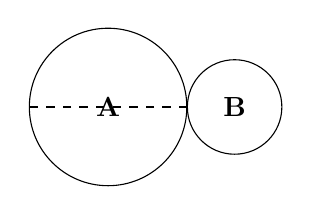
\begin{tikzpicture}
    \node[
    circle,
    draw,
    text = black,
    minimum size = 2cm
    ] (p) at (0,0){{\bf A}};
    \draw[thick,dashed] (p.east) to (p.west);
    \node[
    circle,
    draw,
    text = black,
    minimum size = 1.2cm
    ] (p2) at ($(p.east) + (0.6,0)$){{\bf B}};
  \end{tikzpicture}
  \caption{ }\label{fig:sb}
\end{subfigure}%
\begin{subfigure}{.33\textwidth}
  \centering
  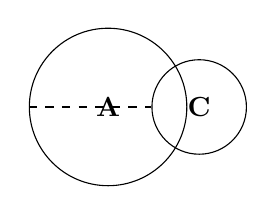
\begin{tikzpicture}
    \node[
    circle,
    draw,
    text = black,
    minimum size = 2cm
    ] (p) at (0,0){{\bf A}};
    \node[
    circle,
    draw,
    text = black,
    minimum size = 1.2cm
    ] (p2) at ($(p.east) + (0.15,0)$){{\bf C}};
    \draw[thick,dashed] (p.west) to (p2.west);
  \end{tikzpicture}
  \caption{ }\label{fig:int}
\end{subfigure}
\begin{subfigure}{.33\textwidth}
  \centering
  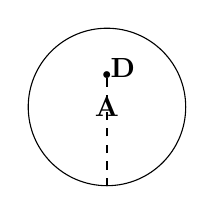
\begin{tikzpicture}
    \node[
    circle,
    draw,
    text = black,
    minimum size = 2cm
    ] (p) at (0,0){{\bf A}};
    \node[] (p2) at (0, .4){\LARGE \bf .};
    \node[] (p3) at (.2, .5){\bf D};
    \draw[thick,dashed] (p.south) to (p|-p2);
  \end{tikzpicture}
  \caption{ }\label{fig:cc}
\end{subfigure}

\end{document}